\documentclass[11pt,a4paper]{article}

\def\X#1{$#1$}

\usepackage[utf8]{inputenc}
\usepackage[danish]{babel}
\usepackage{listings}
\usepackage{color}
\usepackage{graphicx}
\usepackage{float}
\usepackage{textcomp}
\usepackage{amsmath}
\usepackage{verbatim}
\usepackage{array}
\usepackage{textcomp}
\usepackage{fullpage}
\usepackage{pdflscape}
\usepackage{pdfpages}
%\usepackage{hyperref}
\definecolor{listinggray}{gray}{0.9}
\definecolor{lbcolor}{rgb}{0.9,0.9,0.9}
\lstset{
    language=C,
    keywordstyle=\bfseries\ttfamily\color[rgb]{0,0,1},
    identifierstyle=\ttfamily,
    commentstyle=\color[rgb]{0.133,0.545,0.133},
    stringstyle=\ttfamily\color[rgb]{0.627,0.126,0.941},
    showstringspaces=false,
    basicstyle=\footnotesize,
%   numberstyle=\footnotesize,
%   numbers=left,
%   stepnumber=1,
    numbersep=10pt,
    tabsize=2,
    breaklines=true,
    prebreak = \raisebox{0ex}[0ex][0ex]{\ensuremath{\hookleftarrow}},
    breakatwhitespace=false,
    aboveskip={1.0\baselineskip},
    belowskip={1.5\baselineskip},
    columns=fixed,
    upquote=true,
    extendedchars=true,
%   frame=single,
%   backgroundcolor=\color{lbcolor},
}

\title{Automatisk segmentering af mammografier}
\author{Malte Stær Nissen \& Christoffer Hallas Pedersen}

\begin{document}

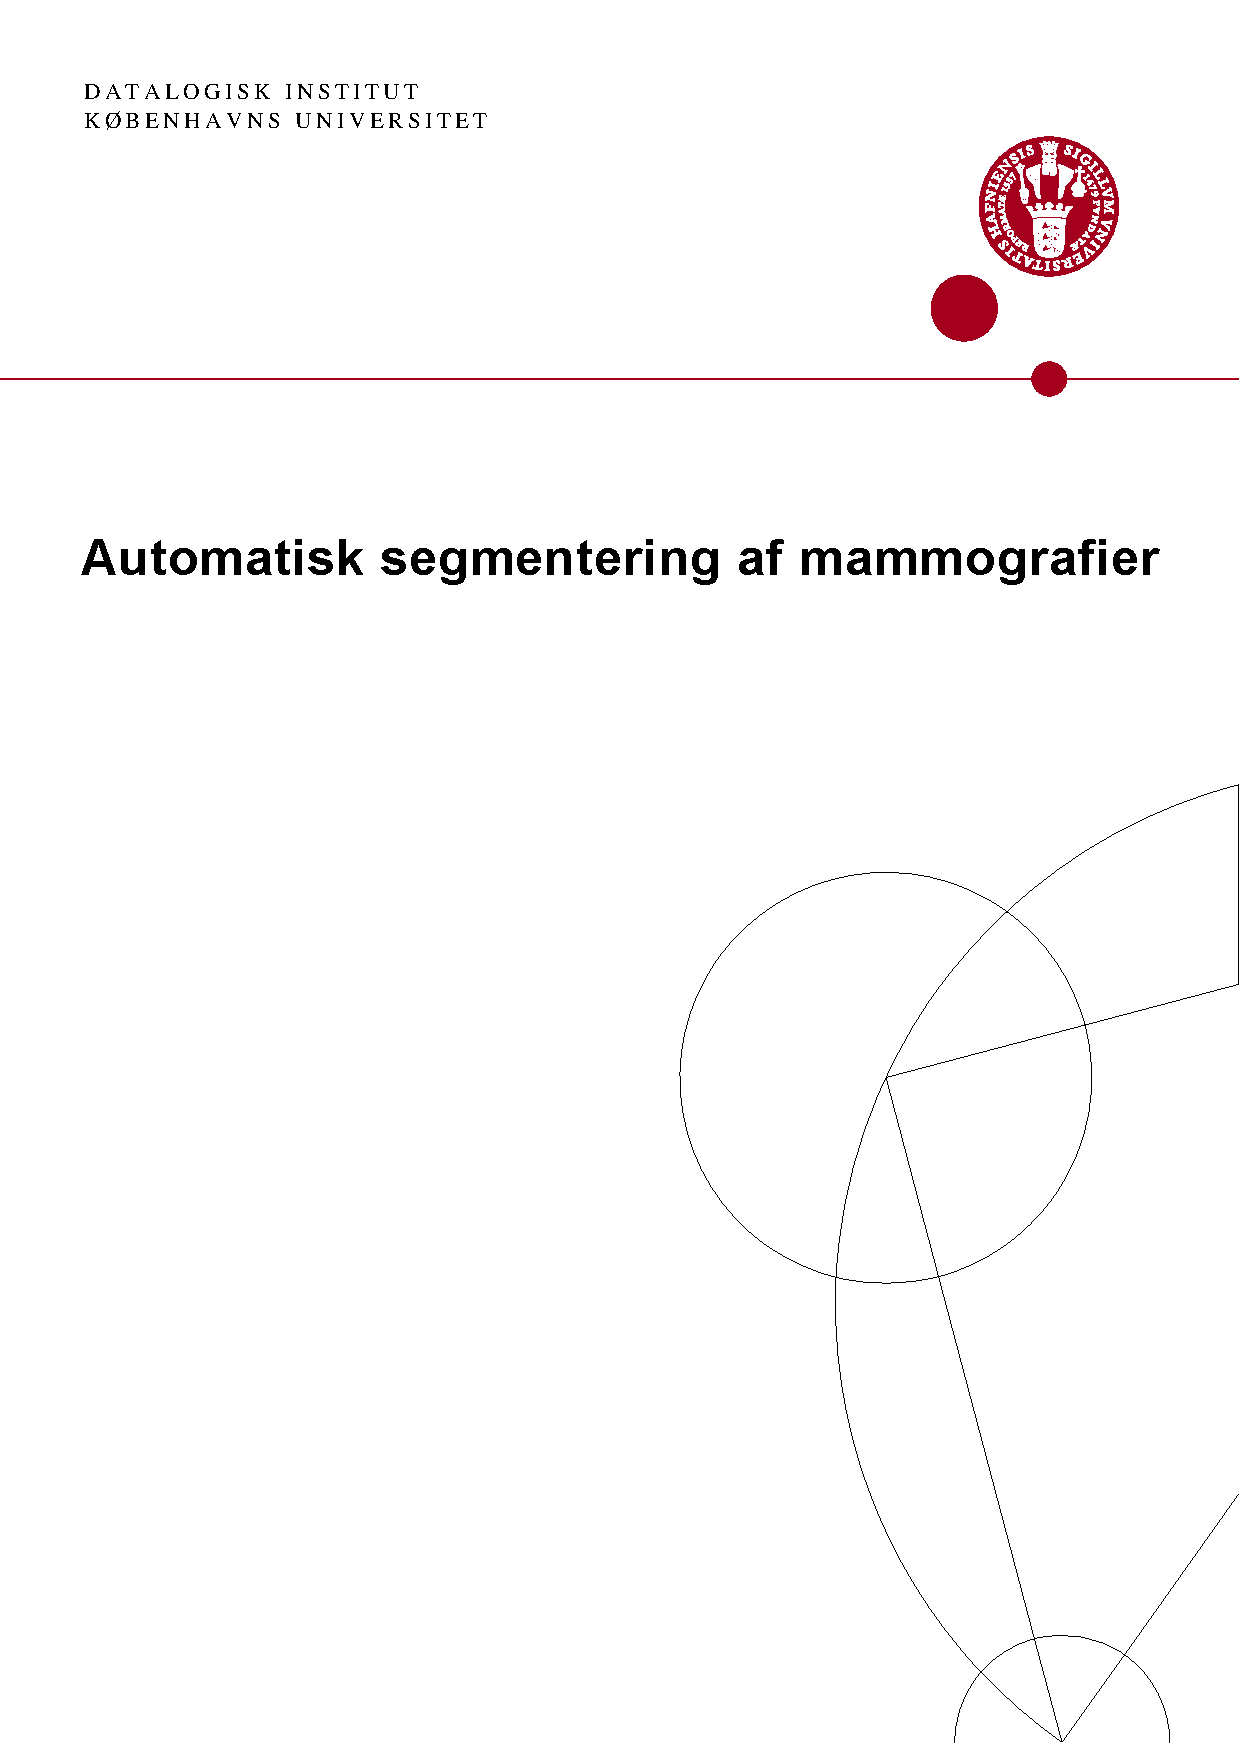
\includepdf{forside.pdf}
\newpage
\clearpage
\pagenumbering{roman}
\tableofcontents

\newpage

\begin{abstract}
\ldots
\end{abstract}

\newpage

\clearpage
\pagenumbering{arabic}

\section{Indledning}

\section{Brystkoordinatsystemet}
Da denne rapport omhandler automatisk segmentering af mammografier, er det naturligt at starte med at beskrive selve segmenteringen af mammografier, før vi begynder at beskrive automatiseringen af denne.

Forskning i detektion af brystcancer er udbredt for tiden, hvorfor der naturligvis bliver udviklet forskellige segmenteringsmetoder. Da man imidlertid er interesseret i ikke blot at kunne sammenligne et mammografi for en patients venstre bryst med det tilsvarende mammografi for det højre bryst, men man derimod ønsker at kunne sammenligne mammografier fra flere patienter og lave statistik over disse, er vi interesserede i at segmentere mammografierne dynamisk. Dette skyldes den naturlige variation i størrelsen samt formen af bryster.

Segmenteringsmetoden, som vi derfor ønsker at automatisere, er beskrevet i \cite{brandtetal}. Denne segmentering går helt basalt ud på at finde de tre punkter $A$, $B$ og $C$. Mammografier viser typisk både en del af brystmuskulaturen samt selve brystvævet på trods af, at man typisk kun ønsker at analysere brystvævet for at forsøge at detektere tegn på brystcancer. Vi ønsker derfor, at brystmuskulaturen så vidt muligt bliver udeladt fra vores segmentering. 

Brystmuskulaturen kan have forskellige former fra patient til patient, men det er typisk muligt at modellere grænsen mellem brystmuskulaturen og brystvævet som en tilnærmelsesvis lige linje. Vi definerer derfor en lige linje på brystmuskulaturens kant (pektorallinjen). Selve grænsen mellem brystvævet og baggrunden har typisk form som en parabel, hvorfor vi definerer en parabelbrystgrænse ved en approksimation. Punkterne $B$ og $C$ definerer vi da som de to skæringspunkter mellem pektorallinjen og parabelbrystgrænsen. Da brystvorten og dermed også punktet $A$ naturligvis ligger enten direkte på parabelbrystgrænsen eller meget tæt på denne, men brystvorten generelt er svær at identificere på mammografier, definerer vi blot punktet $A$ som det punkt på parabelbrystgrænsen, der ligger længst væk fra pektorallinjen. Figur~\ref{fig:bks}, side~\pageref{fig:bks} viser et eksempel på identifikationen af $A$, $B$ og $C$, hvor den gule linje viser brystvævets afgrænsninger og de røde stiplede linjer viser koordinatsystemets afgrænsninger.

De netop beskrevne punkter $A$, $B$ og $C$, er de punkter, som vi ønsker at finde automatisk. Disse punkter danner grundlaget for den efterfølgende dynamiske segmentering, som vi imidlertid ikke ønsker at beskæftige os med.

\begin{figure}
	\centering
		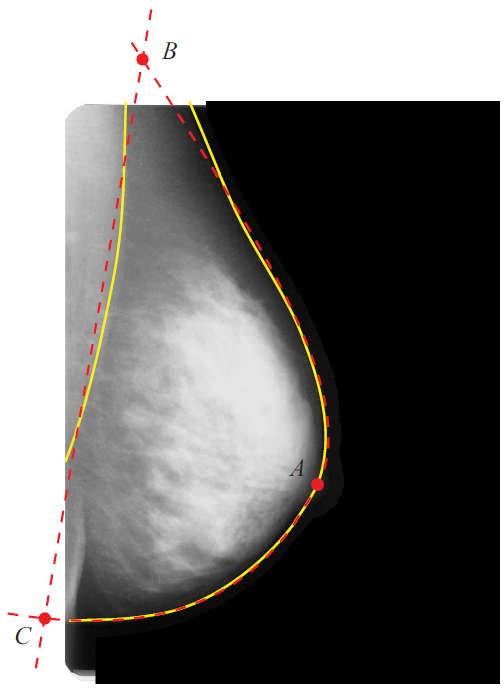
\includegraphics{grafik/brystkoordinatsystem.png}
	\caption{Illustration af brystkoordinatsystemet, fra \cite{brandtetal}, Fig. 1, side 5. De gule linjer viser brystvævets afgrænsninger og de røde stiplede linjer viser koordinatsystemets afgrænsninger}
	\label{fig:bks}
\end{figure}

\section{Den overordnede proces}
\ldots

\section{Simpel detektion af kantpunkter}

\section{Hough transformation}
\ldots

\section{Diskussion om succesmetrikken}
\ldots

\section{Test og sammenligning af implementeringen}
\ldots

\section{Konklusion}
\ldots

\bibliographystyle{plain}
\bibliography{referencer}

\end{document}
